%%%%%%%%%%%%%%%%%%%%%%%%%%%%%%%%%%%%%%%%%%%
\documentclass[11pt, a4paper, twoside]{article}
\usepackage[utf8]{inputenc}
\usepackage[T1]{fontenc}
\usepackage[english]{babel}
\usepackage{lmodern}
\usepackage{geometry}
\geometry{hmargin=2cm,vmargin=2cm}
\usepackage{graphicx}

\usepackage{xcolor}
\usepackage{calrsfs} %% for nice calligraphic letters

\usepackage{dsfont}
\usepackage{amsmath}
\usepackage{amssymb}
\usepackage{amsthm}
\usepackage{enumitem}
\usepackage{parskip}
\usepackage{comment}

\usepackage{fancyvrb} % for verbatim for code

\usepackage{dsfont}
\usepackage{caption}
\captionsetup[figure]{labelfont=bf} % for title figures
\usepackage{hyperref} % to reference the figures
\usepackage{float} % to fix the figure placement with option [H]
\usepackage{subcaption} %  for subfigures environments
%%%%%%%%%%%%%%%%%%%%%%%%%%%%%%%%%%%%%%%%%%%
\newcommand{\floor}[1]{\lfloor #1 \rfloor} % partie entière

\newcommand{\N}{\mathbb{N}} % nb naturels
\newcommand{\Z}{\mathbb{Z}} % entiers relatifs
\newcommand{\R}{\mathbb{R}} % c'est réel
\newcommand{\Q}{\mathbb{Q}} % nb rationnels
\renewcommand{\P}{\mathbb{P}} % nb premiers ou proba
\newcommand{\vp}{\varphi}
\newcommand{\eps}{\varepsilon}
\newcommand{\inv}{^{-1}}
\newcommand{\ind}{\mathds{1}} % indicatrice

\newcommand{\rest}[1]{\raise-.5ex\hbox{\ensuremath|}_{#1}} % restriction
\newcommand{\grad}{\nabla} % gradient
\renewcommand{\div}{\text{div}} % divergence

\newcommand{\Ltwo}{L^2(\Omega)}
\newcommand{\Linf}{L^\infty(\Omega)}
\newcommand{\Hun}{H^1(\Omega)}
\newcommand{\Hunz}{H^1_0(\Omega)}
\newcommand{\Cinfz}{C^\infty_0(\Omega)}
\newcommand{\intom}{\int_\Omega}
\newcommand{\intbd}{\oint_{\partial \Omega}}
\renewcommand{\d}{\text{d}}

\newcommand{\norm}[2]{|| #2||_{#1}}

\newcommand{\st}{such that }
\newcommand{\ie}{i.e. }
\newcommand{\wrt}{with respect to }
\newcommand{\sub}{\subseteq}

%%%%%%%%%%%%%%%%%%%%%%%%%%%%%%%%%%%%%%%%%%%

\begin{document}
\title{Project 3: A semilinear elliptic equation}
\author{Estelle Baup and Samuel Bélisle}
\date{Spring 2023}
\maketitle 

%%%%%%%%%%%%%%%%%%%%%%%%%%%%%%%%%%%%%%%%%%%
\section*{Question 1}
%%%%%%%%%%%%%%%%%%%%%%%%%%%%%%%%%%%%%%%%%%%
Take $\alpha > 0$ and $f : \Omega \to \R$.
We want to find the weak formulation to the problem of finding $u_{n+1}$ satisfying the problem
$$\begin{cases}  - \Delta u_{n+1} + \alpha u_n^2 u_{n+1} = f & \text{in } \Omega,\\
u_{n+1} = 0 &\text{on } \partial\Omega,
\end{cases}$$
where $u_n : \Omega \to \R$ is fixed, representing the current iterate, with $u_n = 0$ on $\partial\Omega$.

\subsection*{Weak form}
We multiply by a test function $v\in \Hunz$ and integrate over $\Omega$ to obtain:
$$\intom \left( -\Delta u_{n+1} v + \alpha u_n^2 u_{n+1} v \right) = \intom fv .$$
We use integration by parts to rewrite the left hand side:
\begin{align*}
 \intom (-\Delta u_{n+1} v)
 &= - \intom \div(\grad u_{n+1} v) + \intom \grad u_{n+1} \grad v
 	&\text{by integration by part}
 \\%%%%%%%%%%%%%
 &= - \intbd v (\grad u_{n+1} \cdot \vec n) + \intom \grad u_{n+1} \grad v
 	&\text{by the divergence theorem}
 \\%%%%%%%%%%%%%
 &=  \intom \grad u_{n+1} \grad v
 	&\text{because } v\in\Hunz,
\end{align*}
where we denote $\vec n$ the outer normal vector on the boundary $\partial \Omega$.

The weak formulation is:
\begin{equation}
\label{weak_f} \tag{E1}
\intom
\grad u_{n+1} \grad \phi
+ 
\intom
\alpha u_n^2 u_{n+1} \phi
= \intom f\phi
\quad \forall \phi \in\Hunz.
\end{equation}

We have a stiffness integral, a mass integral with the reaction term $\alpha u_n^2$, as well as a Poisson right hand side.

%%%%%%%%%%%%%%%%%%%%%%%%%%%%%%%%%%%%%%%%%%
\section*{Question 2}
%%%%%%%%%%%%%%%%%%%%%%%%%%%%%%%%%%%%%%%%%%%
We here focus on the fixed-point scheme as presented in the precedent section.

The code for our implementation of this scheme is in the files \verb+integrate.py+ and \verb+Project_SEZAM.py+. The scheme is run by the function \verb+fixed_point_method()+ of the file  \verb+Project_SEZAM.py+ , which needs as parameters the value of $\alpha$, the mesh size, and two arbitrary stropping conditions; We stop when the difference between two iterates is below a given treshold or after a given number of iterations. If that number of iteration treshold is attained before the difference gets low enough, we plot the last iterates. This allowed us to debug the code when it was not working correctly, and can help spot cycling behaviours.

We used a mesh size of $h=0.05$ to ensure that the mesh contains more than 100 vertices, and the given threshold of $10^{-6}$. We also set the maximum of iterations to 20 or 500, chosen to be sure to observe a convergence of our scheme at some step, but avoid letting the program run too much if some code or parameter mistake is made.

For $\alpha=0.1$, the difference value $||u_n -u_{n+1}||_\infty$ drops below $10^{-6}$ after 11 iterations. We obtain the figures \ref{q2fig1}  and \ref{q2fig2} below, by running \verb+fixed_point_method(0.1, 10e-6, 20, 0.05)+.

\begin{figure}[H]
\begin{subfigure}[h]{0.5\linewidth}
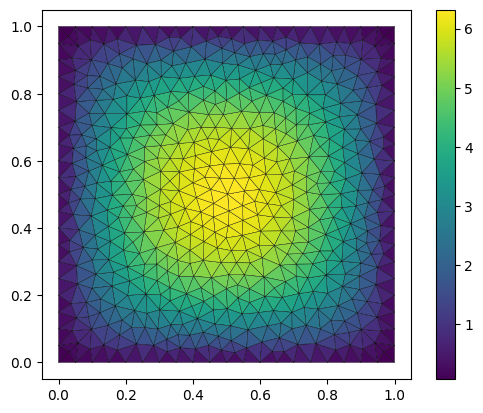
\includegraphics[scale = 0.6]{../Figures/fixed_sol_alpha0.1.png}
\caption{Solution.}
\label{q2fig1}
\end{subfigure}
\hfill
\begin{subfigure}[h]{0.5\linewidth}
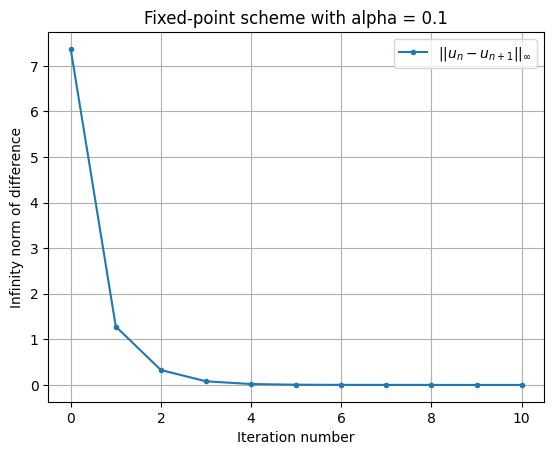
\includegraphics[scale = 0.6]{../Figures/fixed_conv_alpha0.1.png}
\caption{Convergence.}
\label{q2fig2}
\end{subfigure}%
\caption{Solution and convergence rate of the fixed-point scheme for $\alpha=0.1$}
\end{figure}

%%%%%%%%%%%%%%%%%%%%%%%%%%%%%%%%%%%%%%%%%%%

 For $\alpha=2$, $||u_n -u_{n+1}||_\infty$  drops below $10^{-6}$ after 360 iterations, which is much longer. We obtain the figures \ref{q2fig3} and \ref{q2fig4} by running \verb+fixed_point_method(2, 10e-6, 500, 0.05)+.
 
 
\begin{figure}[H]
\begin{subfigure}[h]{0.5\linewidth}
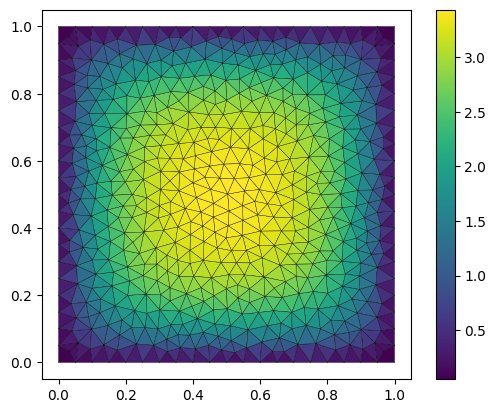
\includegraphics[scale = 0.6]{../Figures/fixed_sol_alpha2.png}
\caption{Solution.}
\label{q2fig3}
\end{subfigure}
\hfill
\begin{subfigure}[h]{0.5\linewidth}
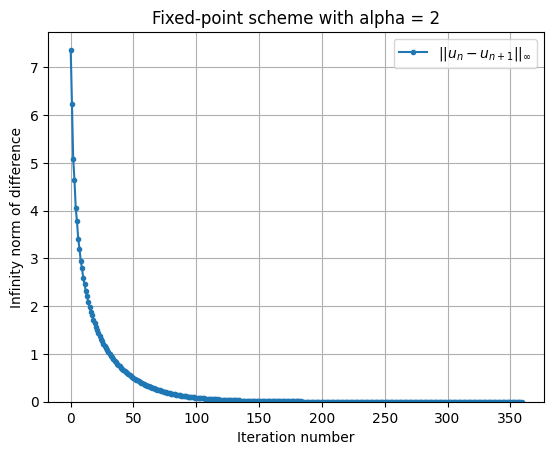
\includegraphics[scale = 0.6]{../Figures/fixed_conv_alpha2.png}
\caption{Convergence.}
\label{q2fig4}
\end{subfigure}%
\caption{Solution and convergence rate of the fixed-point scheme for $\alpha=2$}
\end{figure}

%%%%%%%%%%%%%%%%%%%%%%%%%%%%%%%%%%%%%%%%%%%
\newpage
\section*{Question 3}
In hope to get a better convergence rate, we implemented the Newton scheme as indicated in the project sheet and below.

The code for our implementation of is in the same files \verb+integrate.py+ and \verb+Project_SEZAM.py+. The function that runs the scheme is \verb+newton_method()+, which takes the same parameters as the function for the fixed-point scheme (cf Question 2).
At each iteration, we need to search $\partial u_n$ that satisfies 
\begin{align*}
\intom \grad \phi \cdot \grad \partial u_n + 3\alpha u_n^2 \phi \partial u_n \d\Omega
&= - \intom \grad \phi \cdot \grad u_n + \phi (\alpha u_n^3 - f) \d\Omega \quad
&\forall \phi\in \Hunz,
\\%%%%%%%%%%%%%%%%%%%%%%%%%%%%%%%%%%%%%%
\partial u_n &= 0 \quad
&\text{on } \partial\Omega.
\end{align*}

This is a problem with the same stiffness and mass integrals, except for the reaction term that becomes $3\alpha u_n^2$. The main complication is the right hand side.

Then, we seek the solution $u$ as the limit of the recursive sequence $u_{n+1} =u_n + \partial u_n$.
The solution $\partial u_n$ is computed with the function \verb+newton_iteration()+.
%%%%%%%%%%%%%%%%%%%%%%%%%%%%%%%%%%%%%%%%%%%

For $\alpha = 0.1$, we obtain $||u_n -u_{n+1}||_\infty < 10^{-6}$ after 5 iterations, the solution and convergence rate are shown in figure \ref{q3fig1} and \ref{q3fig2} below, obtained after running \verb+newton_method(0.1, 10e-6, 20, 0.05)+.

\begin{figure}[H]
\begin{subfigure}[h]{0.5\linewidth}
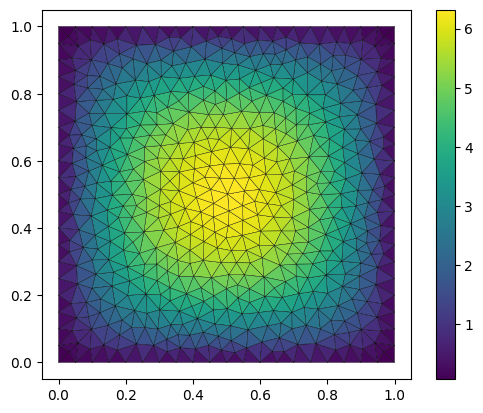
\includegraphics[scale = 0.6]{../Figures/newt_sol_alpha0.1.png}
\caption{Solution.}
\label{q3fig1}
\end{subfigure}
\hfill
\begin{subfigure}[h]{0.5\linewidth}
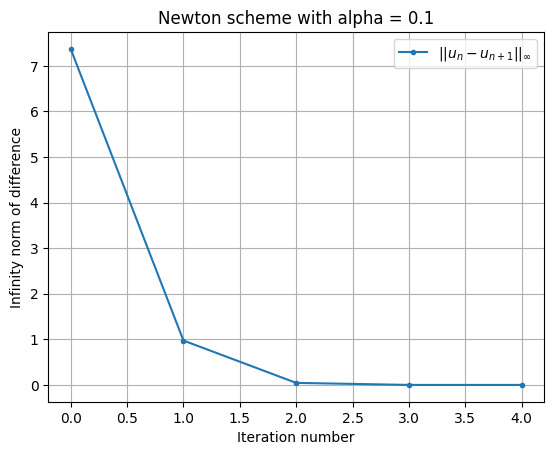
\includegraphics[scale = 0.6]{../Figures/newt_conv_alpha0.1.png}
\caption{Convergence.}
\label{q3fig2}
\end{subfigure}%
\caption{Solution and convergence rate of the Newton scheme for $\alpha=0.1$}
\end{figure}

We see that we find the same solution as with the fixed-point method (see figure \ref{q2fig1}), and we just needed 5 less iterations with the Newton scheme compared to the fixed-point scheme.\\

%%%%%%%%%%%%%%%%%%%%%%%%%%%%%%%%%%%%%%%%%%%

For $\alpha=2$, we converge in 7 iterations, which is considerably faster than with the fixed-point scheme (we needed 360 iterations to converge with this scheme). We obtain the following results by running \verb+newton_method(2, 10e-6, 20, 0.05)+:

\begin{figure}[H]
\begin{subfigure}[h]{0.5\linewidth}
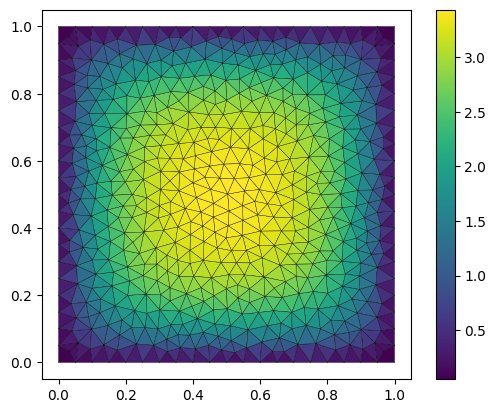
\includegraphics[scale = 0.6]{../Figures/newt_sol_alpha2.png}
\caption{Solution.}
\label{q3fig3}
\end{subfigure}
\hfill
\begin{subfigure}[h]{0.5\linewidth}
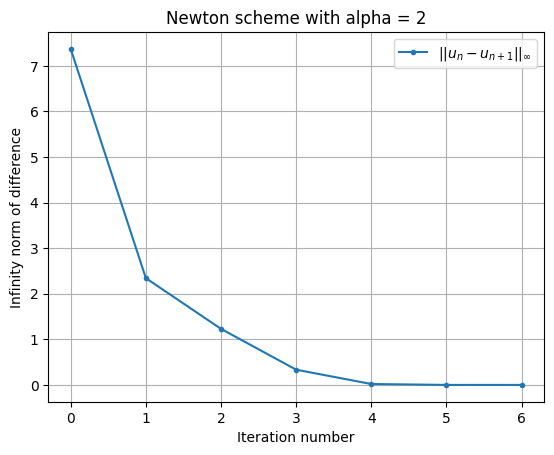
\includegraphics[scale = 0.6]{../Figures/newt_conv_alpha2.png}
\caption{Convergence.}
\label{q3fig4}
\end{subfigure}%
\caption{Solution and convergence rate of the Newton scheme for $\alpha=2$}
\end{figure}

We also see that the solutions are the same for both scheme (figure \ref{q3fig3} above is the same as figure \ref{q2fig3}).\\

%%%%%%%%%%%%%%%%%%%%%%%%%%%%%%%%%%%%%%%%%%%

For $\alpha=5$, we also converge in 7 iterations, and obtain the results shown in figures \ref{q3fig5} and \ref{q3fig6} below (by running \verb+newton_method(5, 10e-6, 20, 0.05)+).

\begin{figure}[H]
\begin{subfigure}[h]{0.5\linewidth}
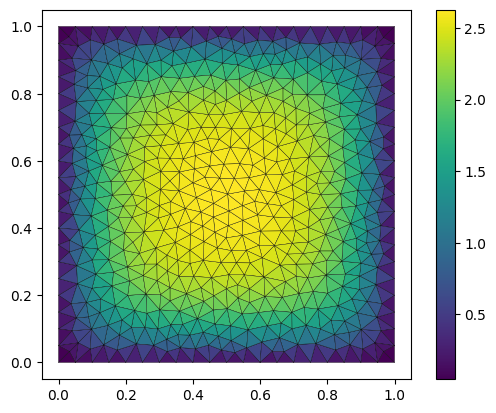
\includegraphics[scale = 0.6]{../Figures/newt_sol_alpha5.png}
\caption{Solution.}
\label{q3fig5}
\end{subfigure}
\hfill
\begin{subfigure}[h]{0.5\linewidth}
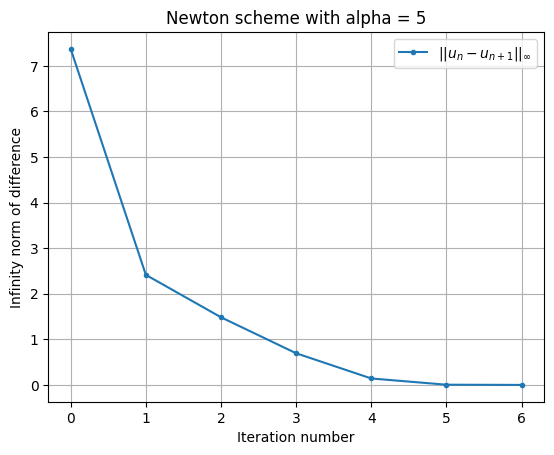
\includegraphics[scale = 0.6]{../Figures/newt_conv_alpha5.png}
\caption{Convergence.}
\label{q3fig6}
\end{subfigure}%
\caption{Solution and convergence rate of the Newton scheme for $\alpha=5$}
\end{figure}

The Newton scheme fares much better than the fixed-point scheme. The number of iterations to obtain $||u_n -u_{n+1}||_\infty < 10^{-6}$ is considerably smaller. (We also ran the scheme for $\alpha=100$, and found that it converges in 10 iterations.)

In the main function of \verb+Project_SEZAM.py+, there is a bonus call, with a smaller grid, just to show off that the scheme converges quickly, even though our implementation is not optimized for it. For instance, we calculate the mass matrix from scratch at each iteration, although it is always the same.

%%%%%%%%%%%%%%%%%%%%%%%%%%%%%%%%%%%%%%%%%%%

\end{document}
